This section focuses on explaining how the system will be deployed, describing the machines involved in the system and what components they will run or contain.

\begin{figure}[H]
	\centering
	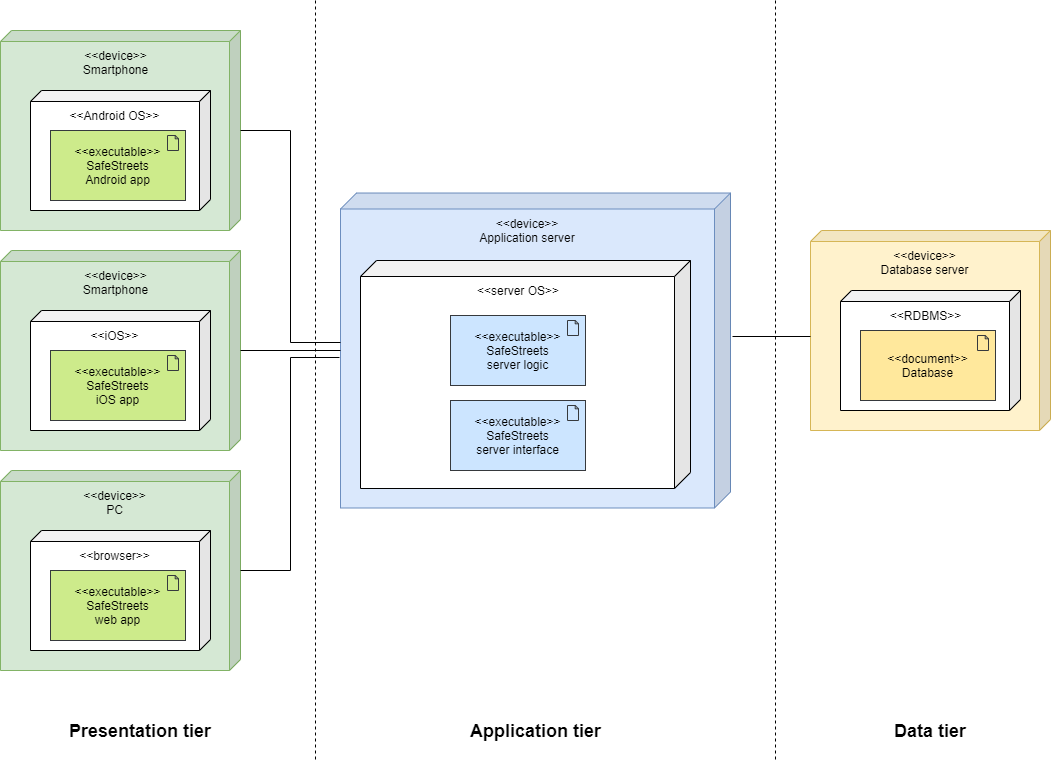
\includegraphics[width=\linewidth]{deploymentDiagram.png}
	\caption{Deployment diagram.}
\end{figure}

In the presentation tier, clients devices will run mobile apps on both Android and iOS smartphones, instead personal computers can run the web application if the user has access to a municipality's account. We decided to implement mobile apps for smartphones to cover citizens and authorities needs of interacting with SafeStreets system in an easy and fast way, because both categories of users will use the apps during their normal routines and it's nowadays common to have a smartphone with you all the time. For municipality instead we choose to implement a web application optimized for desktops, because a municipality member will probably use the software in his workplace, so using a computer is optimal for the task and having a larger layout, with a better level of details when retrieving data, is surely an appreciated feature. A web application is preferred to a website because municipalities will be interested in data research and possible improvements of unsafe areas, so the possibility to filter content and dynamically display and retrieve data is a must. To access the web application, the only requirements is to have a web browser that supports AJAX, so no restrictive requirements are necessary for running it, making it really easy to integrate the use of the software in workflows of every municipality.

In the application tier, the application server structure will be developed internally but deployed on an external hosting service, because internalizing the management of an array of servers is costly and time consuming, while hosting services are nowadays quite cheap, provide assistance and externalize interventions and maintenance. The server needs to provide a REST API to clients and an appropriate backend logic for handling each type of request correctly. Components used by the server are listed and explained widely in section 2.2, so we focus now on server technology. The server structure will be replicated on an array of machines, handled by a load manager for distributing the workload equally and avoid system congestion.

In the data tier, the database is deployed along with its DBMS. The database will be distributed in various instances to improve performances and improve the reliability of the storage. The database server, like the application one, will be hosted on an external service because a specialized service can perform maintenance and provide higher level of support, avoiding SafeStreets team to worry about these topics. A relational DBMS is preferred for the system, because the data is structured and query performance is important for data analysis.
